\documentclass[12pt]{article}
\usepackage[paper=a4paper,left=30mm,right=30mm,top=35mm,bottom =35mm]{geometry}
\usepackage[utf8]{inputenc}
\usepackage[T1]{fontenc}
\usepackage{stmaryrd}
\usepackage{setspace}
\usepackage{mathrsfs}
\usepackage[ngerman]{babel}
\usepackage{amssymb}
\usepackage{amsmath}
\usepackage{fancyhdr}
\usepackage[dvips,unicode,colorlinks,linkcolor=black]{hyperref} 
\usepackage{graphicx}
\usepackage{float}

\pagestyle{fancy}
\lfoot{}
\rfoot{Paul Kremser, Tobias Grussenmeyer}
\cfoot{\thepage}
\fancyhead[L]{FPI Versuch: Faraday- und Pockels-Effekt}
\renewcommand{\headrulewidth}{0.6pt}
\renewcommand{\footrulewidth}{0.6pt}
\setlength{\headheight}{16pt}
\setlength{\parindent}{0pt}
% Für die Wahl der Schriftart
\newcommand{\changefont}[3]{
\fontfamily{#1} \fontseries{#2} \fontshape{#3} \selectfont}

\begin{document}
% keine Hurenkinder und Schusterjungen
\clubpenalty = 10000
\widowpenalty = 10000 
\displaywidowpenalty = 10000

\onehalfspacing
% Schriftart
\changefont{ptm}{m}{n} 

\begin{titlepage}
\author{Paul Kremser, Tobias Grussenmeyer}
\title{Versuch: Faraday- und Pockels-Effekt}
\date{Versuchsdurchführung: 29. Oktober 2009} 
\maketitle
\thispagestyle{empty}
\end{titlepage}


\tableofcontents
\thispagestyle{empty}
\newpage
\pagenumbering{arabic}
\section{Überblick}
Faraday- und Pockelseffekt stellen Möglichkeiten dar einen Lichtstrahl zu beeinflussen. Insbesonere Lässt sich die Intensität verändern. Dies wird in vielen technischen Anwendunen ausgenutzt z.B. LCD-Display. In diesem Versuch sollen der Pockelseffekt anhand von Ammoniumdihydrogenphosphat Kristallen und der Faradayeffekt mittels Schwerflintglas untersucht werden.
\section{Aufgabestellung}

\section{Theoretische Grundlagen}

\subsection{Pockelseffekt}

Bei manchen Kristallen oder Flüssigkeiten ändert sich der Brechungsindex, bezüglich einer bestimmten Richtung, durch anlegen eines elektrischen Feldes. Dieses Phänomen wird als elektrooptischer Effekt bezeichnet. Beim Pockelseffekt hängt die Phasenverschiebung zwischen zwei bestimmten Polarisationskomponenten des hindurchtretenden Lichtes linear von der angelegten Spannung ab. Der Pockelseffekt wird deshalb auch linearer optischer Effekt genannt.\\

Physikalisch wird der Pockelseffekt durch die Doppelbrechung erklärt.
Als \textbf{Doppelbrechung} wird die Eigenschaft von anisotropen Materialien bezeichnet, ein Lichtbündel in zwei senkrecht zueinander polarisierte Teilbündel aufzuspalten. Die Ursache dieses Effekts liegt in unterschiedlichen Brechzahlen in Abhängigkeit von der Ausbreitungsrichtung und Polarisation des Lichtes.

Solche optisch anisotropen Materialien zeichnen sich dadurch aus, dass sie verschiedene Brechzahlen für verschiedene Polarisationen und Richtungen des eingestrahlten Lichtes aufweisen. Dies lässt sich mit dem Brechzahl-Ellipsoid darstellen. Dieses Ellipsoid kann ein Rotationsellipsoid, oder drei verschiedene Hauptachsen besitzen. \\

In optisch einachsigen Kristallen breitet sich der ordentliche Strahl, dessen elektrisches Feld immer senkrecht zur optischen Achse des Kristalls schwingt, wie in einem nicht doppelbrechenden Material aus, ist also transversal zur Ausbreitungsrichtung. Dagegen hat das elektrische Feld des außerordentlichen Strahls, der senkrecht zum ordentlichen polarisiert ist, eine Komponente parallel zur Ausbreitungsrichtung. Beide Komponenten bzgl. der optischen Achse haben unterschiedliche Ausbreitungsgeschwindigkeiten, $(v_{||}$ bzw. $v_{\bot})$, was dazu führt, dass der außerordentliche Strahl im Material bzgl. der Richtung des ordentlichen Strahls etwas geneigt ist.\\

Man kann zu den genannten Geschwindigkeiten Brechzahlen definieren: $n_{ao} = \frac{c}{v_{||}}$, $n_o = \frac{c}{v_{\bot}}$. Die Differenz der Brechzahlen $\Delta n = n_{ao} - n_o$ ist ein Maß für die Doppelbrechung, das Vorzeichen wird als optischer Charakter (oder optische Orientierung) bezeichnet.

In einem positiven einachsigen Kristall, bei dem die Brechzahl des außerordentlichen Strahl $n_{ao}$ größer als die des ordentlichen Strahls $n_o$ ist, bewegt sich der außerordentliche Strahl langsamer als der ordentliche Strahl. Dabei wird die schnelle Achse als die Richtung definiert, in der sich der schneller bewegende Strahl schwingt. Das heißt, in einem positiven einachsigen Kristall ist die „schnelle Achse“ (ordentlicher Strahl) senkrecht zu optischen Achse des Kristalls, während die „langsame Achse“ (außerordentlicher Strahl) mit der optischen Achse übereinstimmt. Für einen negativen einachsigen Kristall stimmt die „schnelle Achse“ mit der optischen Achse überein. \\

\subsubsection[Berechnung des linearen elektrooptischen Koeffizienten]{Berechnung des linearen elekrooptischen Koeffizienten für eine ADP-Pockelszelle in $45^\circ$-Y-Cut}
Das Indexellipsoid für einen ADP-Kristall bei einem angelegten elektrischen Feld ist bis zur ersten Ordunung:
\begin{align}
\label{indexellips}
 \frac{x_1^2}{n_1^2} + 2 r_{41} x_2 E_1 x_3 + \frac{x_2^2}{n_1^2} + 2 r_{41} x_1 E_2 x_3 + \frac{x_3^2}{n_3^2} + 2 r_{63} x_1 x_2 E_3 = 1
\end{align}

Die optische Achse im feldfreien Fall ist hier die $x_3$-Achse. Bei Anlegen des elektrischen Feldes entlang der $x_1$-Achse wird (\ref{indexellips}) zu:


\begin{figure}[H]
\centering
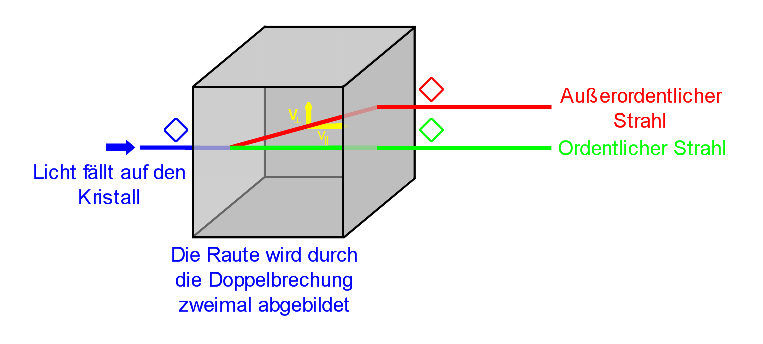
\includegraphics[width=1\linewidth]{pictures/doppelbrechung.eps}
\caption{Doppelbrechung an einem Kristall}
\end{figure}


\section{Versuchsaufbau}

\section{Durchführung}

\section{Auswertung}

\section{Zusammenfassung}

\end{document}
